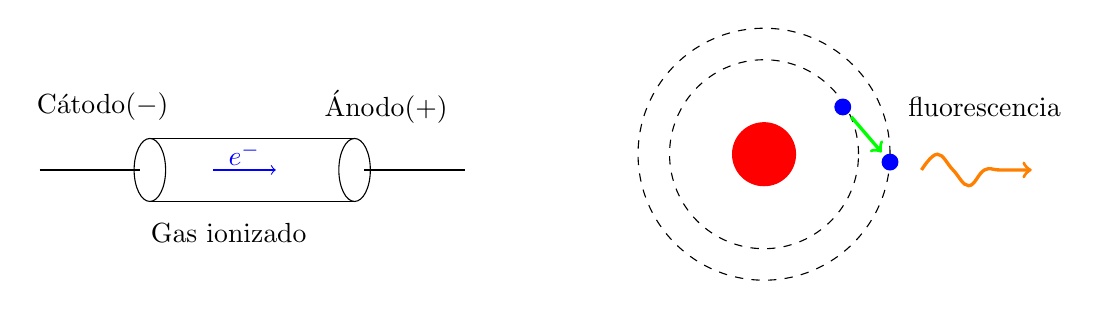
\begin{tikzpicture}

\draw  (-3,0.4) node (v1) {} ellipse (0.2 and 0.4);
\draw  (-0.4,0.4) node (v2) {} ellipse (0.2 and 0.4);
\draw  plot[smooth, tension=.7] coordinates {(-3,0.8) (-0.4,0.8)};
\draw  plot[smooth, tension=.7] coordinates {(-3,0) (-0.4,0)};
\draw [->, blue] plot[smooth, tension=.7] coordinates {(-2.2,0.4) (-1.4,0.4)};
\node at (-3.6,1.2) {C\'atodo($-$)};
\node at (0,1.2) {\'Anodo(+)};
\node at (-2,-0.4) {Gas ionizado};
\draw (-4.4,0.4) -- (v1);
\draw (v2) -- (1,0.4);
\node at (-1.8,0.6) [blue]{$e^-$};
\draw [fill, red] (4.8,0.6) node (v3) {} circle (0.4);
\draw [dashed] (v3) node (v4) {} circle (1.2);
\draw [dashed]  (v4) circle (1.6);
\draw  [fill, blue](5.8,1.2) node (v5) {} circle (0.1);
\draw [fill, blue] (6.4,0.5) node (v6) {} circle (0.1);
\draw [green, ->, very thick](v5) -- (v6);
\node at (7.6,1.2) {fluorescencia};
\draw  [->, orange, very thick]plot[smooth, tension=.7] coordinates {(6.8,0.4) (7,0.6) (7.2,0.4) (7.4,0.2) (7.6,0.4) (7.8,0.4) (8.2,0.4)};
\end{tikzpicture}